\begin{lstlisting}[language=Alloy, caption={Complete Alloy Model for BestBikePaths}, label={lst:alloy_model}]
module BestBikePathsUnified

/* ==============================================================================
   1. DATA TYPES AND ENUMERATIONS
   Defines basic domains: geographic locations, visibility states, 
   road surface conditions, and boolean values for flags.
   ============================================================================== */
sig Location {}

enum PathStatus { Private, Public }
enum Condition { Optimal, Sufficient, Bad }
enum Bool { True, False }

/* ==============================================================================
   2. SYSTEM ACTORS
   The User is the central entity who owns activities (recordings), 
   paths (publications), and leaves feedback.
   ============================================================================== */
sig User {
    myActivities: set Activity,
    myPaths: set Path,
    myFeedbacks: set Feedback
}

/* ==============================================================================
   3. CORE ENTITIES
   ============================================================================== */

/* ENTITY: ACTIVITY (Sensing/Partner Logic)
   Represents raw sensor data recording.
   - trace: the GPS sequence.
   - avgSpeed: used to filter if the activity is actually "biking".
   - sensorAnomalies: potholes automatically detected by accelerometer.
*/
sig Activity {
    owner: one User,
    trace: seq Location,
    avgSpeed: Int,
    sensorAnomalies: set Location
}

/* ENTITY: PATH (Structure and Publishing Logic)
   Represents the consolidated path in the system.
   - trajectory: the geometry of the path.
   - status/isConfirmed: manage the lifecycle (draft -> public).
   - currentCondition: the aggregated state of the path quality.
*/
sig Path {
    owner: one User,
    trajectory: seq Location,
    status: one PathStatus,
    isConfirmed: one Bool,
    currentCondition: one Condition,
    receivedFeedbacks: set Feedback
}

/* ENTITY: FEEDBACK (Community Logic)
   Represents user opinion on a public path.
   Links an author to a target path, specifying conditions and localized obstacles.
*/
sig Feedback {
    author: one User,
    targetPath: one Path,
    reportedCondition: one Condition,
    reportedObstacles: set Location
}

/* ==============================================================================
   4. FACTS (INVARIANTS AND DOMAIN RULES)
   ============================================================================== */

/* FACT: STRUCTURAL CONSISTENCY
   Ensures bidirectional relationships are consistent (e.g., if feedback 
   belongs to a user, it must appear in that user's feedback list) 
   and establishes ownership hierarchy.
*/
fact StructuralConsistency {
    all a: Activity | a in a.owner.myActivities
    all p: Path | p in p.owner.myPaths
    all f: Feedback | f in f.author.myFeedbacks
    all f: Feedback | f in f.targetPath.receivedFeedbacks
}

/* FACT: GEO CONSISTENCY
   Constrains spatial data:
   1. Obstacles reported in feedback must be on the path trajectory.
   2. Anomalies detected by sensors must be on the activity trace.
   Note: .elems converts the sequence to a set for inclusion check.
*/
fact GeoConsistency {
    all f: Feedback | f.reportedObstacles in f.targetPath.trajectory.elems
    all a: Activity | a.sensorAnomalies in a.trace.elems
}

/* FACT: UNIQUE FEEDBACK (Anti-Spam)
   A user can leave at most one feedback per specific path.
   This prevents ranking manipulation by a single actor.
*/
fact UniqueFeedback {
    all p: Path, u: User | lone f: p.receivedFeedbacks | f.author = u
}

/* FACT: ACTIVITY VALIDATION LOGIC (Sensing)
   Defines rules for an activity to become a path:
   If a path is generated from an activity (sharing owner and trace),
   then the average speed must be compatible with biking 
   (here defined between 4 and 12 to stay within Alloy's small integer range).
*/
fact ActivityToPathLogic {
    all p: Path, a: Activity | 
        (p.trajectory = a.trace and p.owner = a.owner) implies {
            a.avgSpeed > 4 
            a.avgSpeed < 12
    }
}

/* FACT: PRIVATE PATH PRIVACY
   If a path is set to Private, no one except the owner can leave feedback 
   or interact with it.
*/
fact PrivatePathPrivacy {
    all f: Feedback | 
        f.targetPath.status = Private implies f.author = f.targetPath.owner
}

\end{lstlisting}



\begin{lstlisting}[language=Alloy, caption={Full Lifecycle Scenario}, label={lst:alloy_model}]

/* ==============================================================================
   5. PREDICATES (TEST SCENARIOS)
   ============================================================================== */

/* SCENARIO 1: THE FULL LIFECYCLE
   Demonstrates the ideal "Happy Path":
   1. A user records a valid activity (correct speed, anomalies detected).
   2. The system generates a path from this activity.
   3. The user confirms and publishes the path.
   4. A different user leaves feedback on the path.
*/
pred FullLifecycleScenario {
    some u1, u2: User | some a: Activity | some p: Path | some f: Feedback | {
        a.owner = u1
        a.avgSpeed = 6 
        #a.sensorAnomalies > 0 
        
        p.owner = u1
        p.trajectory = a.trace
        
        p.isConfirmed = True
        p.status = Public
        
        f.author = u2
        u1 != u2 
        f.targetPath = p
        f.reportedCondition = Bad 
        
        #p.trajectory > 2 
    }
}
run FullLifecycleScenario for 5 but 5 Int

\end{lstlisting}

\begin{figure}[H] % [H] forza l'immagine esattamente in questo punto
    \centering
    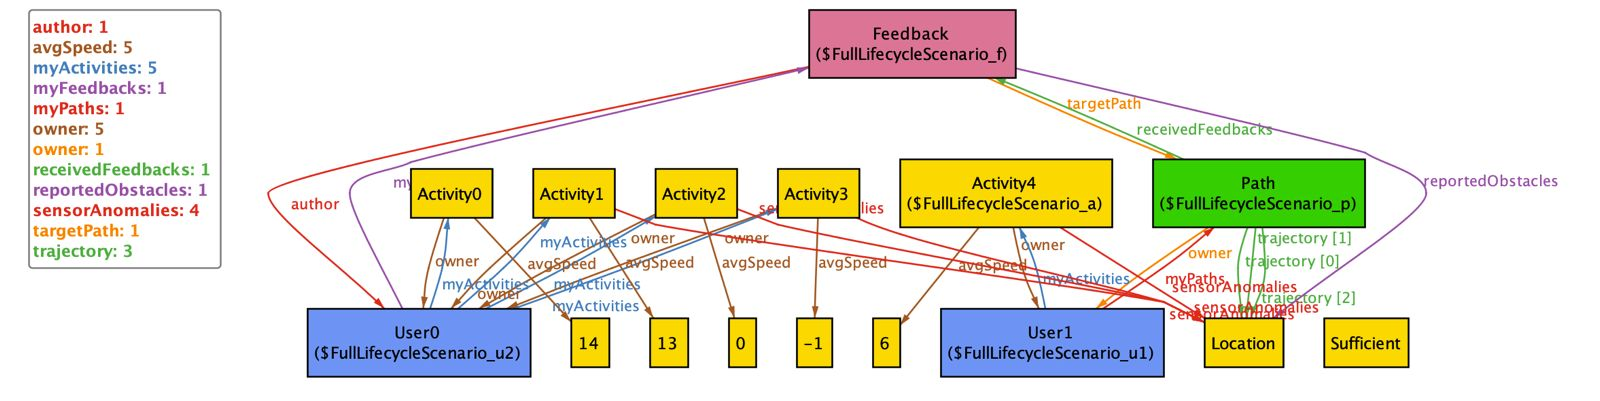
\includegraphics[width=0.8\textwidth]{Images/full_lifecycle_graph_1.jpeg} 
    \caption{Alloy instance: Full Lifecycle Scenario.}
    \label{fig:alloy_instance_1}
\end{figure}
\begin{figure}[H] % [H] forza l'immagine esattamente in questo punto
    \centering
    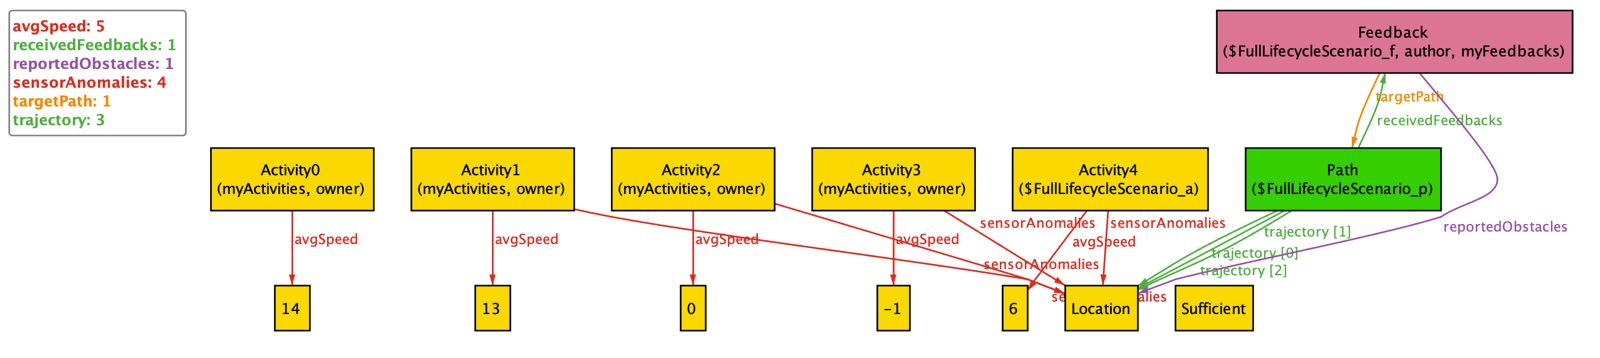
\includegraphics[width=0.8\textwidth]{Images/full_lifecycle_graph_2.jpeg} 
    \caption{Alloy instance: Full Lifecycle Scenario Projection User0.}
    \label{fig:alloy_instance_1}
\end{figure}
\begin{figure}[H] % [H] forza l'immagine esattamente in questo punto
    \centering
    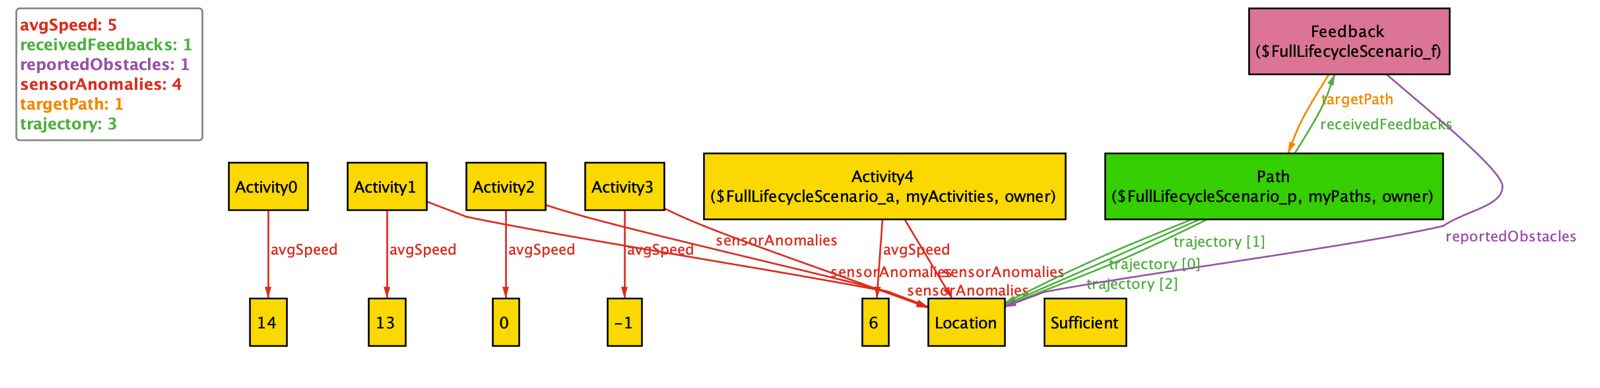
\includegraphics[width=0.8\textwidth]{Images/full_lifecycle_graph_3.jpeg} 
    \caption{Alloy instance: Full Lifecycle Scenario Projection User1.}
    \label{fig:alloy_instance_1}
\end{figure}

\section{Confliting Feedback Merge Scenario}

\begin{lstlisting}[language=Alloy, caption={Confliting Feedback Merge Scenario}, label={lst:alloy_model}]
    /* SCENARIO 2: CONFLICTING FEEDBACK MERGE
    Verifies that the system supports divergent opinions.
    Generates a public path with at least two feedbacks reporting 
    opposite conditions (e.g., Optimal vs Bad).
    */
    pred ConflictingFeedbackMerge {
        some p: Path | {
            p.status = Public
            #p.receivedFeedbacks >= 2
            some disj f1, f2: p.receivedFeedbacks | {
                f1.reportedCondition = Optimal
                f2.reportedCondition = Bad
            }
        }
    }
    run ConflictingFeedbackMerge for 4 but 5 Int
\end{lstlisting}

This scenario demonstrates the system's capability to handle and persist divergent opinions from the community regarding the same public path, a necessary condition for the merging logic.
The generated instance depicts a single Path with Public status linked to multiple distinct Feedback entities. Specifically, the model enforces the existence of conflicting reports, where one user rates the condition as Optimal while another rates it as Bad. 
This scenario formally validates the structural prerequisites for the Data Merging requirement. It proves that the domain model allows for the coexistence of contradictory data points without inconsistency. This accumulation of diverse feedback is the input required by the server-side aggregation algorithm to dynamically compute the path's overall score and \texttt{currentCondition}. 

\begin{figure}[H] % [H] forza l'immagine esattamente in questo punto
    \centering
    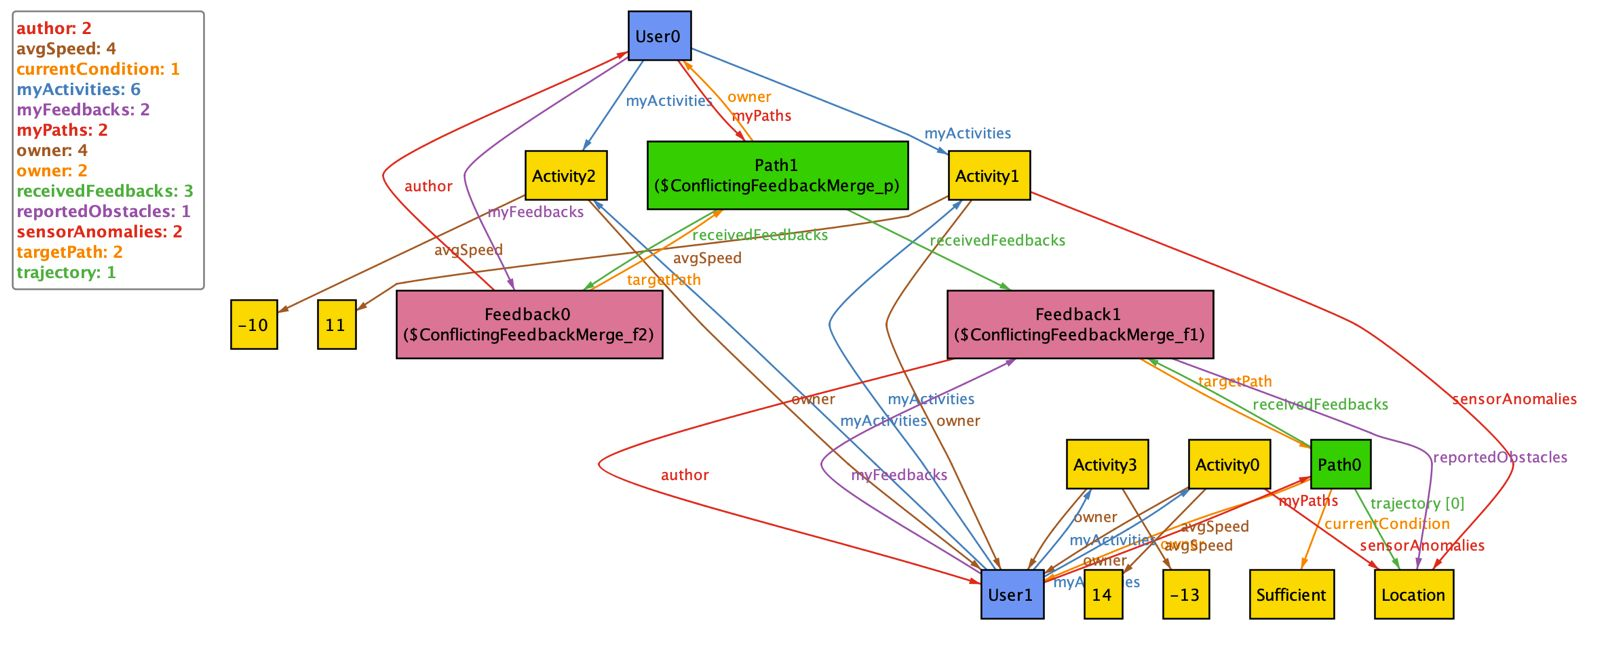
\includegraphics[width=0.8\textwidth]{Images/conflict_feedback_merge_graph.jpeg} 
    \caption{Alloy instance: Conflicting Feedback Merge Scenario.}
    \label{fig:alloy_instance_4}
\end{figure}

\section{Rejected Activity Filter Scenario}

\begin{lstlisting}[language=Alloy, caption={Rejected Activity Filter Scenario}, label={lst:alloy_model}]
/* SCENARIO 3: REJECTED ACTIVITY FILTER
   Demonstrates system robustness (Safety).
   Verifies the existence of an activity that is too slow (e.g., walking at speed 3)
   and ensures that NO path is generated from it.
*/
pred RejectedActivityScenario {
    some a: Activity | {
        a.avgSpeed = 3 
        
        no p: Path | p.owner = a.owner and p.trajectory = a.trace
    }
}
run RejectedActivityScenario for 3 but 5 Int
\end{lstlisting}

This scenario serves as a negative test to verify the robustness of the system's filtering logic, ensuring that invalid activities do not pollute the path database.
The predicate simulates an edge case where an Activity is recorded with an \texttt{avgSpeed} of 3 (representing a walking pace), which falls below the mandatory threshold defined in the domain facts (speed >4). The solver confirms that, in this state, no Path entity sharing the same trace and owner exists. 
This successfully verifies the Safety and Data Integrity constraints. It demonstrates that the logical rules correctly prevent the promotion of non-cycling activities (e.g., walking or running) into public paths, thereby guaranteeing that the platform remains focused exclusively on biking data. 

\begin{figure}[H] % [H] forza l'immagine esattamente in questo punto
    \centering
    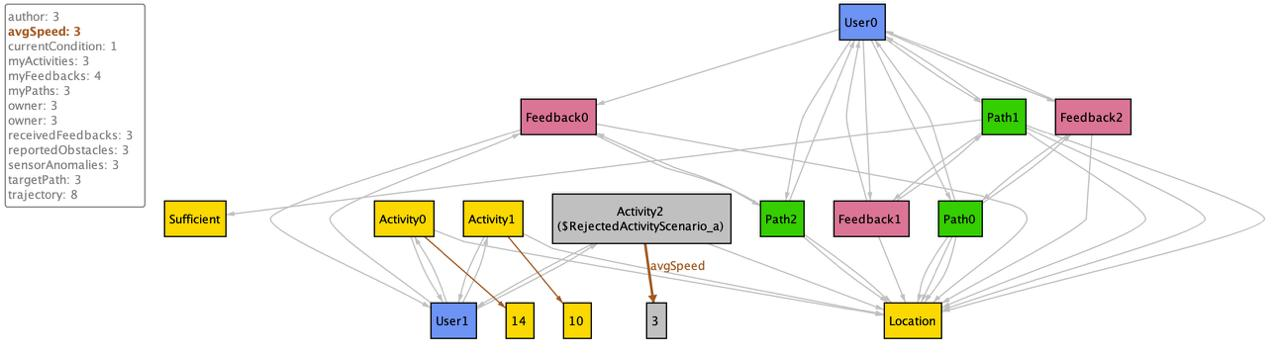
\includegraphics[width=0.8\textwidth]{Images/rejected_activity_graph.jpeg} 
    \caption{Alloy instance: Rejected Activity Scenario.}
    \label{fig:alloy_instance_5}
\end{figure}